An important notion to introduce when processing data and designing features for use in machine learning or signal processing, is that the amount of information, or entropy, contained in a data source depends not only on its size but also on the presence of patterns such as mutual information between latent variables and periodicity in series. In the present \textit{Big Data} context this rarely enters as a problem of information scarcity, but rather as a source of error due to the risk of capturing uninformative patterns in the feature design, which may go unobserved thus leading to false conclusions. To give an intuition of how this can cause problems, consider the following example.\\

\texttt{feature A} measures the fraction of time a user is looking at his or her phone while socially engaged, and \texttt{feature B} measures the unique number of friends that the user has through a given period. If one were to plot the distribution of these variables for a set of individuals against eachother, it would yield an almost perfect inverse correlation, begging the interpretation that looking at your phone while socially engaged means you have less friends. The problem with this analysis is that \texttt{feature A} is normalized by the summed time socially engaged, which unsurprisingly correlates with \texttt{feature B}. The consequence is that the latent variable the analyst is trying to get at, namely the propensity to interact with one's phone while social, vanishes in product with a variable that so strongly correlates with the target. At the same time, removing the normalization term creates the inverse problem, because the summed time of phone use while socially engaged necessarily depends on how much a user engages socially and thereby number of unique friends. In the given case, a better design of \texttt{feature A} would be to measure the \textit{amount of phone use while socially engaged vs. while alone} in which case it should behave independently from other features.\\

Uninformative patterns are expected for mathematical, systematic or other boring reasons, and are often undesired since they wash out interesting informative patterns, like in the example given above. Patterns which are considered most informative are those that emerge unexpectedly or in line with a hypothesis and demands explanation only through interpretation or further research. In general, careful consideration must be made to capture mostly patterns that informs the analysis. Features must be designed to cultivate patterns that express properties of the system which are not entirely self-evident. This excludes not only features capturing uninformative patterns, but also a large number of other features we as humans know to be mutually informative or in correlation. Consider how, for a set of individuals, the \textit{number of calls made} vs. \textit{number of calls received} would, aligned with our expectations, be in strong correlation, but that \textit{number of calls made and received} vs. \textit{percent of calls going out}, would not. Both feature pairs are derived from the same call-log data, but as illustrated in Fig. \ref{fig:example_informative_features}, a far more informative pattern is captured with the latter pair.

\begin{figure}[h!]
	\centering
	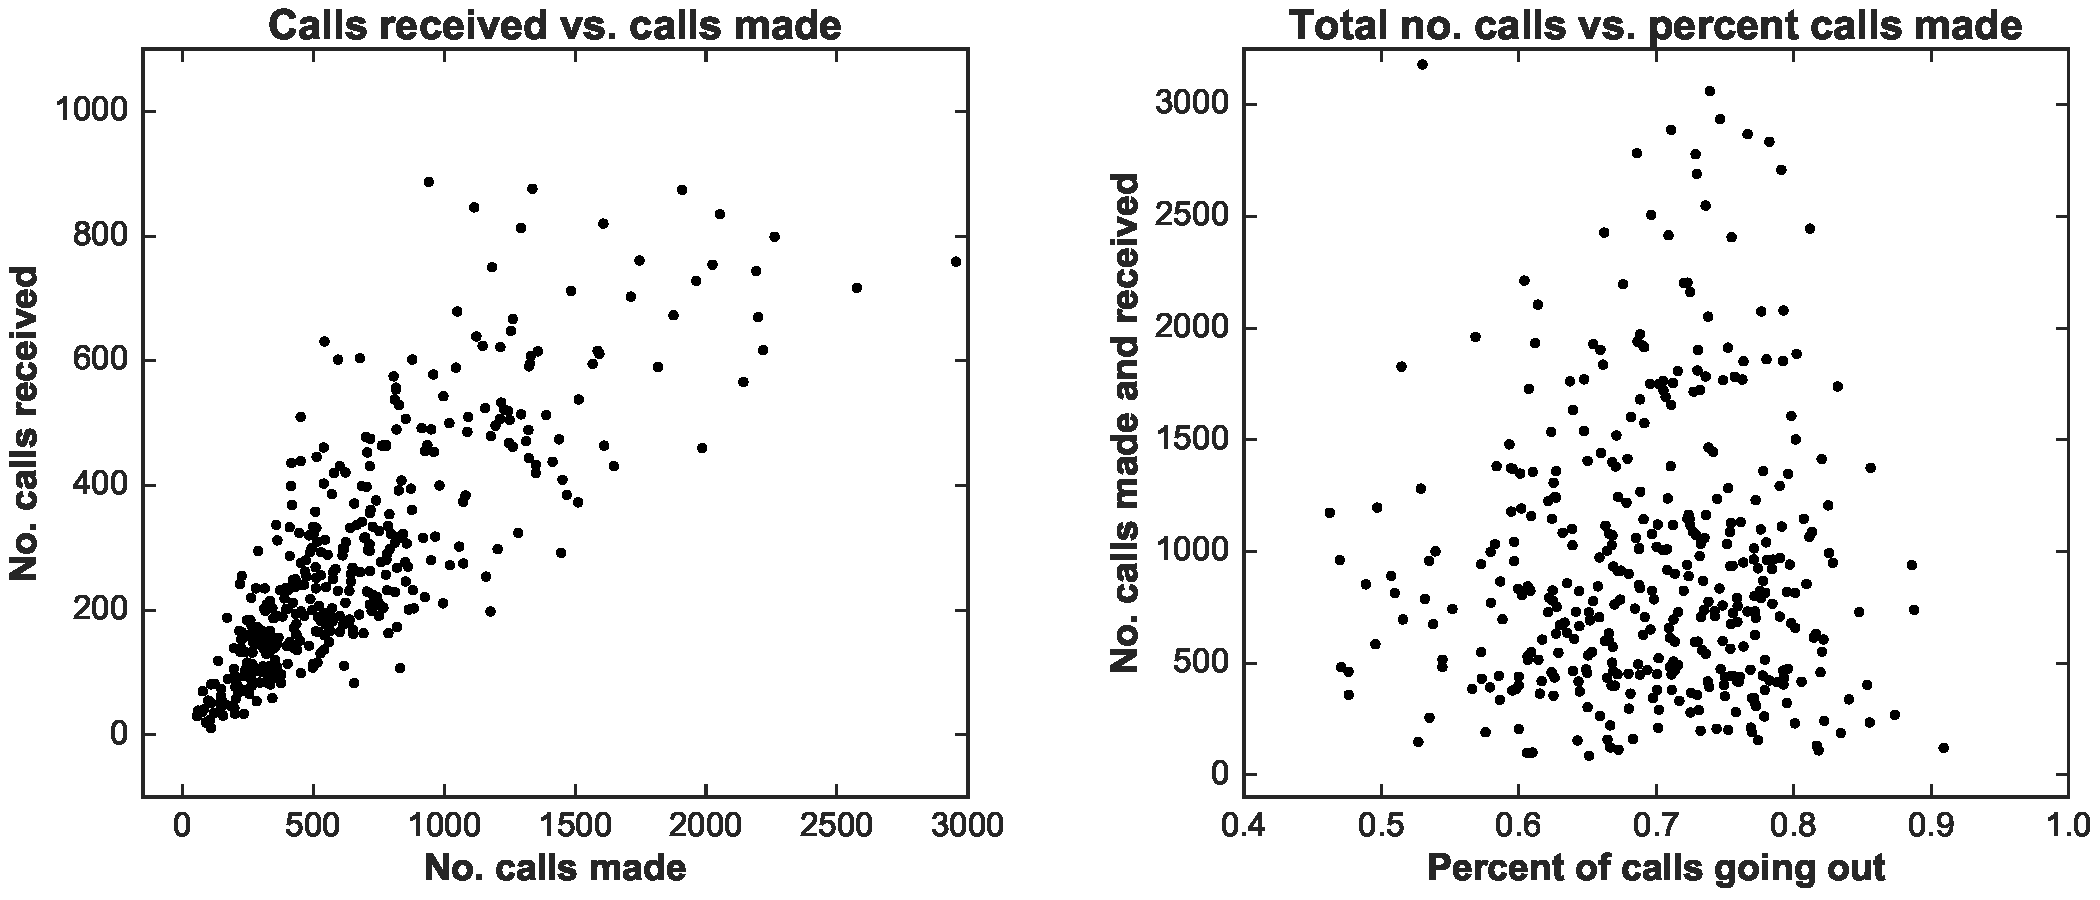
\includegraphics[width=0.9\textwidth]{figures/example_informative_features}
	\caption{\label{fig:example_informative_features} Casting features differently changes the pattern they capture. Each plot represents a different way of casting the same call-log data, but the right one obviously captures a more informative pattern. It allows one to make genuinely interesting observations, such as how only individuals with an outgoing to incoming call ratio between 0.7 and 0.8 make and receive far above average number of calls.}
\end{figure}

In practice it is tedious to engineer features to only capture patterns that inform the analysis. In fact, trying to achieve this often creates problems since the task of developing the necessary complex features requires significantly more coding, which increases the risk of generating uncaught bugs. In this work, it is attempted to strike a balance between the informative and the simple. In other words, great care has been taken to understand the data which has led to the realization that it is not feasible to completely avoid capturing uninformative patterns, and as such features are designed in a way that attempts to minimize these, not exclude them.